

\newproblem{08b}
{
	Graph the line with slope $\dfrac{-2}{3}$ that passes through the point $(2, -1)$. Be sure to label axes with $x$, $y$, and with numbers. Identify at least three points on your line.\begin{onlyproblem}\begin{center}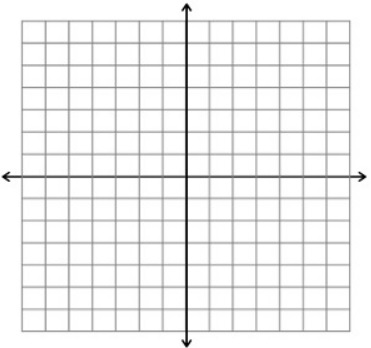
\includegraphics{fig-graphpaper.png}\end{center}\end{onlyproblem} \begin{onlysolution}\begin{center}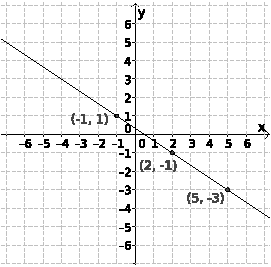
\includegraphics{fig095-08-b-answer}\end{center}\end{onlysolution}
}
{
	\begin{tabular}{l r}
	1 point for correct labeling of axes and numbers on them.\\
	3 points for correctly identifying 3 pts.\\
	1 pt for the correct line.\\
	\end{tabular}
}
